\documentclass[dvipsnames]{beamer}

%% build: latexmk -pdf -pvc -interaction=nonstopmode -xelatex prez.tex

%% general
%% --------------------------------------------------------------------------------
\usepackage{xcolor}
\usepackage{amssymb}
\usepackage{amsmath}
\usepackage{hyperref}
\usepackage{fontspec}
\usepackage{proof}
\usepackage{tikz-cd}

%% Beamer
%% --------------------------------------------------------------------------------
\usetheme{Boadilla}
\setbeamertemplate{navigation symbols}{}
\setbeamertemplate{footline}[frame number]
\setbeamerfont{itemize/enumerate subbody}{size=\normalsize}
\setbeamerfont{itemize/enumerate subsubbody}{size=\normalsize}


%% Bibliography
%% --------------------------------------------------------------------------------
\bibliographystyle{apalike}
\setbeamerfont{bibliography item}{size=\footnotesize}
\setbeamerfont{bibliography entry author}{size=\footnotesize}
\setbeamerfont{bibliography entry title}{size=\footnotesize}
\setbeamerfont{bibliography entry location}{size=\footnotesize}
\setbeamerfont{bibliography entry note}{size=\footnotesize}
\setbeamertemplate{bibliography item}{}

%% Monofont
%%--------------------------------------------------------------------------------
\setmonofont[Scale=1.0]{DejaVu Sans Mono}

%% square dot
\makeatletter
\DeclareRobustCommand{\sqcdot}{\mathbin{\mathpalette\morphic@sqcdot\relax}}
\newcommand{\morphic@sqcdot}[2]{%
  \sbox\z@{$\m@th#1\centerdot$}%
  \ht\z@=.33333\ht\z@
  \vcenter{\box\z@}%
}
\makeatother


%% --------------------------------------------------------------------------------
% this file is needed to build telescopes.tex

%% %% setting \sqcdot as HoTT-book-style transitivity
%% \makeatletter
%% \DeclareRobustCommand{\sqcdot}{\mathbin{\mathpalette\morphic@sqcdot\relax}}
%% \newcommand{\morphic@sqcdot}[2]{%
%%   \sbox\z@{$\m@th#1\centerdot$}%
%%   \ht\z@=.33333\ht\z@
%%   \vcenter{\box\z@}%
%% }
%% \makeatother


\renewcommand{\U}{\mathsf{U}}
\newcommand{\El}{\mathsf{El}}
\newcommand{\REN}{\mathsf{REN}}
\newcommand{\op}{\mathsf{op}}
\newcommand{\ra}{\rightarrow}
\newcommand{\Ra}{\Rightarrow}

\newcommand{\Set}{\mathsf{Set}}
\newcommand{\PSh}{\mathsf{PSh}}
\newcommand{\FamPSh}{\mathsf{FamPSh}}
\renewcommand{\ll}{\llbracket}
\providecommand{\rr}{\rrbracket}
\newcommand{\Con}{\mathsf{Con}}
\newcommand{\Ty}{\mathsf{Ty}}
\newcommand{\Tm}{\mathsf{Tm}}
\newcommand{\Tms}{\mathsf{Tms}}
\newcommand{\R}{\mathsf{R}}
\newcommand{\TM}{\mathsf{TM}}
\newcommand{\NE}{\mathsf{NE}}
\newcommand{\NF}{\mathsf{NF}}
\newcommand{\p}{\mathsf{p}}
\newcommand{\q}{\mathsf{q}}
\renewcommand{\u}{\mathsf{u}}
\renewcommand{\ne}{\mathsf{ne}}
\newcommand{\nf}{\mathsf{nf}}
\newcommand{\lQ}{\mathsf{lQ}}
\newcommand{\lU}{\mathsf{lU}}
\renewcommand{\lq}{\mathsf{lq}}
\newcommand{\lu}{\mathsf{lu}}
\newcommand{\cul}{\ulcorner}
\newcommand{\cur}{\urcorner}
\newcommand{\norm}{\mathsf{norm}}
\newcommand{\Nf}{\mathsf{Nf}}
\newcommand{\Ne}{\mathsf{Ne}}
\newcommand{\Nfs}{\mathsf{Nfs}}
\newcommand{\Nes}{\mathsf{Nes}}
\newcommand{\ID}{\mathsf{ID}}
\newcommand{\id}{\mathsf{id}}
\newcommand{\nat}{\,\dot{\rightarrow}\,}
%\newcommand{\nat}{\overset{\mathsf{n}}{\ra}} % this is how we denote it in the formalisation
\newcommand{\Nat}{\mathsf{Nat}}
\renewcommand{\S}{\overset{\mathsf{s}}{\ra}} % we have it with uppercase S in the formalisation
\newcommand{\blank}{\mathord{\hspace{1pt}\text{--}\hspace{1pt}}} %from the book
%\newcommand{\blank}{\!{-}\!}
\newcommand{\lam}{\mathsf{lam}}
\newcommand{\app}{\mathsf{app}}
\newcommand{\tr}[2]{\ensuremath{{}_{#1 *}\mathopen{}{#2}\mathclose{}}}
\renewcommand{\C}{\mathsf{C}}
\newcommand{\Code}{\mathsf{Code}}
\renewcommand{\M}{\mathsf{M}}
% from the book
%\newcommand{\M}{{\scalebox{0.6}{$\mathsf{M}$}}}
%% \newcommand{\C}{\mathcal{C}}
\newcommand{\data}{\mathsf{data}}
\newcommand{\ind}{\hspace{1em}}
\newcommand{\idP}{\mathsf{idP}}
\newcommand{\compP}{\mathsf{compP}}
\newcommand{\idF}{\mathsf{idF}}
\newcommand{\compF}{\mathsf{compF}}
\newcommand{\proj}{\mathsf{proj}}
\newcommand{\ExpPSh}{\mathsf{ExpPSh}}
\newcommand{\map}{\mathsf{map}}
\newcommand{\Var}{\mathsf{Var}}
\newcommand{\Vars}{\mathsf{Vars}}
\newcommand{\wk}{\mathsf{wk}}
\newcommand{\neuU}{\mathsf{neuU}}
\newcommand{\neuEl}{\mathsf{neuEl}}
\newcommand{\var}{\mathsf{var}}
\newcommand{\natn}{\mathsf{natn}}
\newcommand{\natS}{\mathsf{natS}}
\newcommand{\LET}{\mathsf{let}}
\newcommand{\IN}{\mathsf{in}}
\newcommand{\refl}{\mathsf{refl}}
\newcommand{\trans}{\mathbin{\raisebox{0.2ex}{$\displaystyle\centerdot$}}}
\newcommand{\zero}{\mathsf{zero}}
\newcommand{\suc}{\mathsf{suc}}
\newcommand{\N}{\mathbb{N}}

\newcommand\arcfrombottom{
  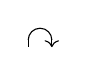
\begin{tikzpicture}[scale=0.03em]
    \draw (0,0) arc (0:180:0.5);
    \draw (0,0) edge[->] (0,-0.3);
    \draw (-1,0) edge (-1,-0.3);
  \end{tikzpicture}
}
\newcommand\arcfromtop{
  
\begin{tikzpicture}[scale=0.03em]
    \draw (0,0) arc (180:360:0.5);
    \draw (0,0) edge[->] (0,0.3);
    \draw (1,0) edge (1,0.3);
  \end{tikzpicture}
}

\newcommand{\Elim}{\mathsf{Elim}}
\newcommand{\elim}{\mathsf{elim}}
\newcommand{\Rec}{\mathsf{Rec}}
\newcommand{\record}{\mathsf{record}}
\newcommand{\funext}{\mathsf{funext}} \newcommand{\Q}{\mathsf{Q}}
\renewcommand{\T}{\mathsf{T}} \newcommand{\leaf}{\mathsf{leaf}}
\newcommand{\node}{\mathsf{node}} \newcommand{\perm}{\mathsf{perm}}
\newcommand{\coe}{\mathsf{coe}} \newcommand{\vz}{\mathsf{vz}}
\newcommand{\vs}{\mathsf{vs}} \newcommand{\untr}{\mathsf{untr}}
\newcommand{\from}{\mathsf{from}}
\newcommand{\fromeq}{{\mathsf{from}\hspace{-0.3em}\equiv}}
\newcommand{\fromsimeq}{{\mathsf{from}\hspace{-0.3em}\simeq}}
\newcommand{\Model}{\mathsf{Model}}
\newcommand{\DModel}{\mathsf{DModel}}
\newcommand{\module}{\mathsf{module}}
\newcommand{\open}{\mathsf{open}}
\renewcommand{\P}{\mathsf{P}} \newcommand{\Bool}{\mathsf{Bool}}
\newcommand{\true}{\mathsf{true}} \newcommand{\false}{\mathsf{false}}
\renewcommand{\not}{\mathsf{not}} \newcommand{\0}{\mathsf{0}}
\newcommand{\1}{\mathsf{1}} \renewcommand{\Pr}{\mathsf{Pr}}
\newcommand{\PrNat}{\mathsf{PrNat}} \newcommand{\J}{\mathsf{J}}
\newcommand{\wkV}{\mathsf{wkV}} \renewcommand{\r}[1]{{\P_{#1}}}
\newcommand{\stab}{\mathsf{stab}} \newcommand{\NTy}{\mathsf{NTy}}
\newcommand{\isDec}{\mathsf{isDec}} \newcommand{\dec}{\mathsf{dec}}
\newcommand{\yes}{\mathsf{yes}} \newcommand{\no}{\mathsf{no}}
\newcommand{\case}{\mathsf{case}} \newcommand{\inj}{\mathsf{inj}}
\newcommand{\K}{\mathsf{K}} \newcommand{\lb}{\langle}
\newcommand{\rb}{\rangle} \newcommand{\Decl}{\mathsf{Decl}}
\newcommand{\Core}{\mathsf{Core}} \newcommand{\IND}{\mathsf{ind}}
\newcommand{\Id}{\mathsf{Id}} \newcommand{\Base}{\mathsf{Base}}
\newcommand{\Setoid}{\mathsf{Setoid}}
\newcommand{\FamSetoid}{\mathsf{FamSetoid}}
\newcommand{\prop}{\mathsf{prop}} \newcommand{\resp}{\mathsf{resp}}
\newcommand{\transport}{\mathsf{transport}}
\newcommand{\I}{\mathsf{I}} \newcommand{\E}{\mathsf{E}}
\newcommand{\transp}{\mathsf{transp}}
\newcommand{\Transp}{\mathsf{Transp}}
\newcommand{\W}{\mathsf{W}}
\newcommand{\Fin}{\mathsf{Fin}} \newcommand{\fzero}{\mathsf{fzero}}
\newcommand{\fsuc}{\mathsf{fsuc}}
\newcommand{\inv}{\mathsf{inv}}
\newcommand{\con}{\mathsf{con}}
\newcommand{\LEFT}{\mathsf{left}}
\newcommand{\RIGHT}{\mathsf{right}}
\newcommand{\seg}{\mathsf{seg}}
\newcommand{\Int}{\mathsf{Int}}
\renewcommand{\in}{\mathbin{\hat:}}
%% \renewcommand{\hat}[1]{{\color{BrickRed}{#1}}}
\newcommand{\vdashh}{\mathbin{\hat\vdash}}
\newcommand{\rah}{\mathbin{\hat\ra}}
\newcommand{\commah}{\hat,\,}
\newcommand{\timesh}{\mathbin{\hat\times}}
\newcommand{\eqh}{\mathbin{\hat=}}
\newcommand{\TR}{\hat{\mathsf{tr}}}
\newcommand{\ap}{\hat{\mathsf{ap}}}
\newcommand{\apd}{\hat{\mathsf{apd}}}
\renewcommand{\tt}{\hat{\mathsf{tt}}}
\newcommand{\Tel}{\hat{\mathsf{Tel}}}
\newcommand{\Type}{\hat{\mathsf{Type}}}
\newcommand{\emptytel}{\hat{\epsilon}}
\newcommand{\telext}{\mathbin{\hat{\lhd}}}
\newcommand{\ltel}{\hat{\ll}}
\newcommand{\rtel}{\hat{\rr}}
\newcommand\pp{\ensuremath{\hat{\mathbin{+\mkern-10mu+}}}}
%% \newcommand{\semicol}{\hat;\,}
%% \newcommand{\targetass}{\hat{\Gamma}\semicol}
%\newcommand{\targetass}{;}

\newcommand{\cR}[1]{{\color{Red}{#1}}}
\newcommand{\targetass}{\cR{\Gamma};}
\newcommand{\semicol}{\cR;\,}
\newcommand{\A}{\mathsf{A}}
\newcommand{\F}{\mathsf{F}}
\newcommand{\D}{\mathsf{D}}
\renewcommand{\S}{\mathsf{S}}


%% --------------------------------------------------------------------------------

%% TODO: adjust beginning (what are HIITs, what is the content of the talk)

%% --------------------------------------------------------------------------------

\title{Inductive types\thanks{This work was supported by the European Union, co-financed by the European
    Social Fund (EFOP-3.6.3-VEKOP-16-2017-00002).}}

\author{András Kovács}
\institute{Eötvös Loránd University, Department of Programming Languages and Compilers}
\date{11 Jan 2019}

%% --------------------------------------------------------------------------------

\AtBeginSection[]
{
  \begin{frame}
    \frametitle{Contents}
    \tableofcontents[currentsection]
  \end{frame}
}


%% --------------------------------------------------------------------------------

\begin{document}

\frame{\titlepage}

\begin{frame}{Introduction}

This talk is a brief introduction to 2018 research on inductive types, by Ambrus
Kaposi and myself, with additional contribution from Thorsten Altenkirch and
Péter Diviánszky. This has been my main EFOP research topic in the past year.
\vspace{1em}

Related talks and publications:

\begin{itemize}
\item Altenkirch, Diviánszky, Kaposi, Kovács: \emph{Constructing inductive-inductive types using a domain-specific type theory}, TYPES 2018
\item Kaposi, Kovács: \emph{A Syntax for Higher
  Inductive-Inductive Types}, FSCD 2018 (award: best paper by junior researchers)
\item Kaposi, Kovács, Altenkirch: \emph{Constructing Quotient Inductive-Inductive Types}, POPL 2019
\end{itemize}

\end{frame}

%% --------------------------------------------------------------------------------

\begin{frame}{Introduction}

  Proof by induction is well-known. However, the concept is often left imprecise.
  Some questions:

  \begin{itemize}
  \item What is exactly an inductive definition?
  \item When is proof by induction valid?
  \item How can we get a precise logical statement of induction for an inductive definition?
  \item What properties should inductive structures have besides having induction principles?
  \end{itemize}

\vspace{1em}
\pause

These are general questions of mathematical foundations, and are not necessarily tied to practical
formal methods.


\end{frame}

\begin{frame}{Examples of inductive definitions}

  \begin{itemize}
  \item Inductive sets: natural numbers, (syntax) trees, lists.
  \item Inductive relations: typing derivations, reduction in
    operational semantics, proof trees for logics.
  \end{itemize}

\pause
\vspace{1em}
\vspace{1em}
Induction on natural numbers or lists is obvious, but induction on typing derivations
is less so. Just writing down the statement of induction can be challenging for
many structures.

\end{frame}


\begin{frame}[fragile]{Common features}


  \begin{itemize}
  \item A collection of sets and families of sets, called sorts.
  \item A collection of production rules (constructors), each producing elements of some set.
  \item The assumption that elements of the sorts are precisely those generated by finitely many
        applications of constructors.
  \end{itemize}

\vspace{1em}
Example with single sort:

\begin{verbatim}
        Nat  : Set
        zero : Nat
        suc  : Nat → Nat
\end{verbatim}
\vspace{1em}
If we allow an infinite number of \texttt{suc}-s, \texttt{Nat}-induction becomes \textbf{false}.

\end{frame}

\begin{frame}[fragile]{Quotient induction}

We may also allow \emph{equations} besides production rules.
\vspace{1em}

Example: a quotient inductive definition of integers.

\begin{verbatim}
        Int     : Set
        zero    : Int
        suc     : Int → Int
        pred    : Int → Int
        sucPred : ∀ i → suc (pred i) = i
        predSuc : ∀ i → pred (suc i) = i
\end{verbatim}

All constructions defined on integers must respect the equations. This is enforced
by the \texttt{Int}-induction principle.
\vspace{1em}

E. g. we cannot define a function from integers such that the results
for \texttt{suc (pred i)} and \texttt{i} are different.

\end{frame}

\begin{frame}[fragile]{Quotient induction}

Quotient induction is a powerful tool for formalizing lots of mathematics, including
\vspace{1em}

\begin{itemize}
\item Real, ordinal, surreal numbers.
\item Syntax and semantics of languages, especially those with polymorphic and dependent types.


\end{itemize}

\pause
\vspace{1em}
No current proof assistant supports quotient inductive types.
\vspace{1em}

A key motivation of this research is to build theoretical background for future proof assistants.
\vspace{1em}

(Besides doing pure theory, we're also writing prototype implementations)


\end{frame}

\begin{frame}{Results on quotient induction}

In the POPL paper.
\vspace{1em}

\begin{itemize}
\item A formal description of valid quotient inductive definitions,
      as typing contexts in a special-purpose type theory.
\item Categorical semantics in rather high detail.
\item Showing that every quotient inductive type can be constructed from just one universal quotient
      inductive type.
\end{itemize}

\end{frame}

\begin{frame}{Results on higher induction}

In the FSCD paper.
\vspace{1em}

\emph{Higher} induction is used to define spaces generated from n-dimensional
constructors (points, paths, surfaces, etc.).  It is a broad generalization of
quotient induction. It's important in homotopy type theory.
\vspace{1em}

A lot more complicated than quotient induction. Accordingly, our results are
significantly weaker for higher induction than for quotient induction.

\end{frame}

\begin{frame}{Future work}
  \begin{itemize}
  \item Modest generalizations of current results.
  \item Write PhD thesis on quotient induction.
  \item Combine research with setoid type theory (reasearch by INRIA Nantes, Ambrus, Thorsten), implement prototype.
  \end{itemize}

\end{frame}


\begin{frame}

  \center{\large{Thank you!}}

\end{frame}

\end{document}
